\appendix{Specyfikacja interfejsów Lupus}\label{appendix:4}

Specyfikacja w formie elektronicznej znajduje się pod linkiem: \url{https://github.com/0x41gawor/lupus/blob/master/docs/spec/lupin-lupout.md}.

\subsection{Architektura}

\begin{figure}[!h]
    \centering 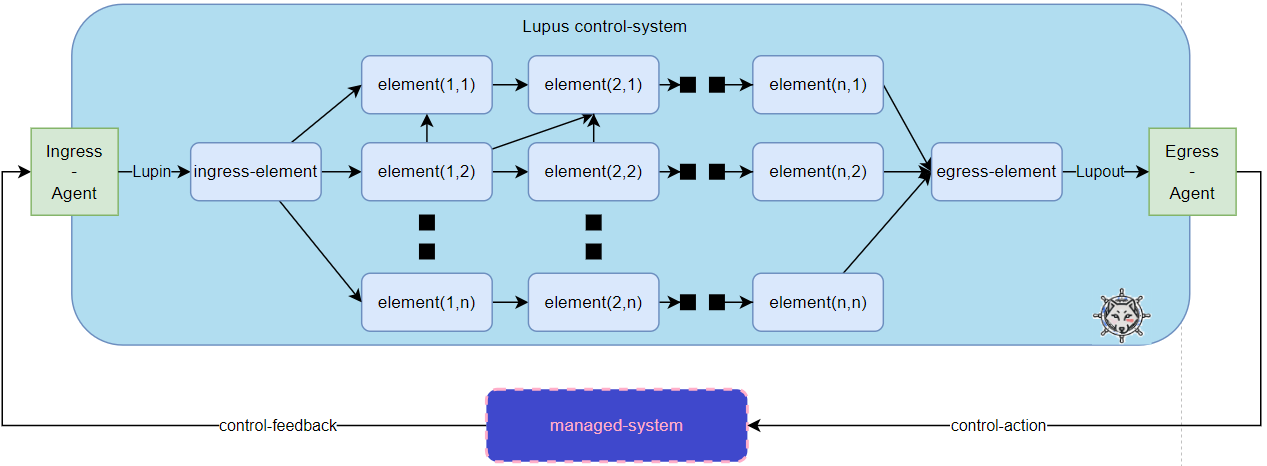
\includegraphics[width=1\linewidth]{a4-arch.png}
    \caption{Architektura Lupus. Źródło: Opracowanie własne.}\label{fig:a4-arch}
\end{figure}

\subsection{Interfejs Lupin}

\hyperlink{def:projektant}{\textbf{Projektant}} może zdefiniować wiele \hyperlink{def:element-lupus}{\textbf{Elementów Lupus}}, połączonych na różne, skomplikowane sposoby. Musi jednak zdecydować, który z nich zostanie wywołany przez \hyperlink{def:agent-ingress}{\textbf{Agenta Ingress}}. Taki element można nazwać \hyperlink{def:element-ingres}{\textbf{Elementem Ingress}}. \hyperlink{def:lupus}{\textbf{Lupus}} zaleca posiadanie tylko jednego \hyperlink{def:element-ingres}{\textbf{Elementu Ingress}}.

Jeśli \hyperlink{def:agent-ingress}{\textbf{Agent Ingress}} chce zasygnalizować, że można zaobserwować nowy stan \hyperlink{def:system-zarzadzany}{\textbf{Systemu Zarządzanego}} (co oznacza, że musi zostać uruchomiona nowa iteracja \hyperlink{def:zamknieta-petla-sterowania}{\textbf{Pętli Sterowania}}), musi zmodyfikować pole \texttt{Status.Input} w \textit{obiekcie API} \hyperlink{def:element-ingres}{\textbf{Elementu Ingress}}. Wartość umieszczona w tym polu będzie reprezentować nowy \hyperlink{def:stan-aktualny}{\textbf{Stan Aktualny}}.

Pole \texttt{Status.Input} w \hyperlink{def:element-ingres}{\textbf{Ingress Element CR}} jest typu \texttt{RawExtension}, co oznacza, że podlega pod specyfikację \hyperlink{def:dane}{\textbf{Danych}} (\hyperref[appendix:5]{Załącznik 5}).

JSON przesłany w tym miejscu będzie stanowił \hyperlink{def:dane}{\textbf{Dane}} dla tego elementu.

Oprogramowanie implementuje interfejs \texttt{Lupin}, jeśli w pewnym miejscu swojego kodu wysyła żądanie HTTP do \textbf{kube-api-server}, które aktualizuje status \hyperlink{def:element-ingres}{\textbf{Elementu Ingress}}, a dokładniej pole \texttt{input}. Wartość musi być obiektem JSON, który reprezentuje \hyperlink{def:stan-aktualny}{\textbf{Aktualny Stan}} \hyperlink{def:system-zarzadzany}{\textbf{Systemu Zarządzanego}}. 

\subsection{Interfejs Lupout}

Punktem wyjścia z \hyperlink{def:system-sterowania}{\textbf{Systemu Sterowania Lupus}} jest ostatni \hyperlink{def:element-lupus}{\textbf{Element Lupus}}, czyli \hyperlink{def:element-egress}{\textbf{Element Egress}}. Wysyła on swoje \hyperlink{def:finalne-dane}{\textbf{Finalne Dane}} (lub ich część) do \hyperlink{def:agent-egress}{\textbf{Agenta Egress}}. \hyperlink{def:agent-egress}{\textbf{Agent Egress}} musi przekształcić to wejście w \hyperlink{def:akcja-sterujaca}{\textbf{Akcję Sterowania}}, wykonywaną bezpośrednio na \hyperlink{def:system-zarzadzany}{\textbf{Systemie Zarządzanym}}.

Oprogramowanie implementuje interfejs \texttt{Lupout}, jeśli implementuje serwer HTTP, który akceptuje wejściowe \hyperlink{def:dane}{\textbf{Dane}} w formacie JSON i tłumaczy je na \hyperlink{def:akcja-sterujaca}{\textbf{Akcję Sterowania}}, wykonywaną na \hyperlink{def:system-zarzadzany}{\textbf{Systemie Zarządzanym}}. 
